\subsubsection{Base de datos.}

El modelo de datos del launcher se compone de seis entidades principales, cada una diseñada para encapsular un aspecto específico de la funcionalidad del launcher:

\begin{itemize}
  \item \textbf{ApplicationsModel:} Entidad para gestionar las aplicaciones instaladas en el dispositivo. Esta almacena información esencial sobre cada aplicación que el usuario puede controlar a través del launcher.
  \item \textbf{TasksModel:} Representa las tareas que el usuario puede crear y gestionar dentro del launcher como parte de su sistema de productividad personal.
  \item \textbf{HabitsModel:} Contiene la información relacionada con los hábitos que el usuario desea formar o mantener como parte de su rutina diaria. Esta entidad sigue una estructura similar a las tareas pero está optimizada para el seguimiento a largo plazo.
  \item \textbf{HabitsLogsModel:} Implementa el sistema de seguimiento temporal para los hábitos, permitiendo el registro histórico del cumplimiento de cada hábito a lo largo del tiempo. Esta implementación permite análisis de tendencias y proporciona al usuario retroalimentación sobre su progreso en la formación de hábitos. Aunque fue implementada, no se utilizó en la versión final del launcher, sino que hace parte de trabajos futuros \textbf{REFERENCIA A TRABAJOS FUTUROS}.
  \item \textbf{CategoriesModel:} Este modelo permite al usuario asignar una etiqueta a tareas y hábitos relacionados.
  \item \textbf{LimitsModel:} Gestiona las restricciones de tiempo que el usuario puede establecer para aplicaciones específicas como parte del sistema de control de uso del dispositivo.
\end{itemize}


La relación entre estas entidades y sus atributos se ilustra en la Figura \ref{fig:diagrama_uml}.

\begin{figure}[ht]
  \caption{Diagrama de la base de datos del launcher.}
  \label{fig:diagrama_uml}
  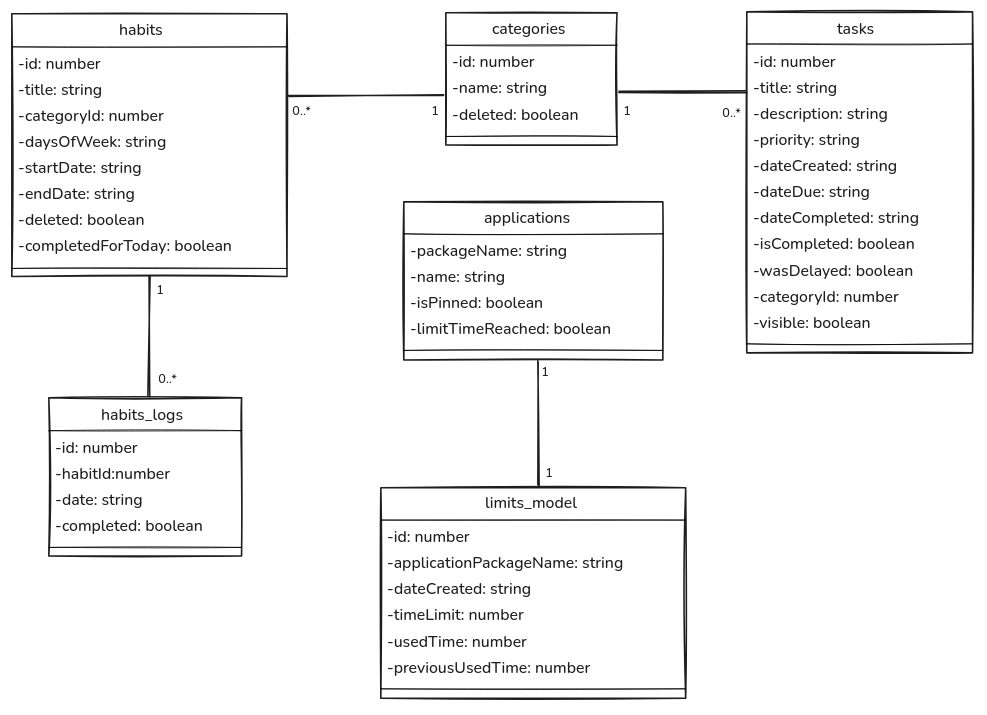
\includegraphics[width=\textwidth]{Figuras/diagrama_uml.png}
  \centering
\end{figure}